\documentclass[11pt]{article}
\usepackage{amsmath}
\usepackage{amssymb}
\usepackage{graphicx}
\usepackage{tikz}
\usetikzlibrary{shapes.geometric, arrows, positioning, fit, backgrounds}
\usepackage{algorithm}
\usepackage{algpseudocode}
\usepackage{geometry}
\usepackage{subcaption}

\geometry{margin=1in}

\tikzstyle{block} = [rectangle, draw, fill=blue!20, text width=6em, text centered, rounded corners, minimum height=3em]
\tikzstyle{data} = [rectangle, draw, fill=green!20, text width=6em, text centered, minimum height=2.5em]
\tikzstyle{process} = [rectangle, draw, fill=orange!20, text width=8em, text centered, rounded corners, minimum height=3em]
\tikzstyle{arrow} = [thick,->,>=stealth]

\title{Radial Basis Function Proxy Model for Well-Based Reservoir Simulation}
\author{}
\date{}

\begin{document}

\maketitle

\section{Overview}

The \texttt{ProxyModelRBF} is a surrogate modeling approach designed to approximate computationally expensive reservoir simulation outputs using Radial Basis Function (RBF) interpolation. This proxy model enables rapid optimization of well control strategies by providing fast predictions of reservoir responses without requiring full physics-based simulations.

\section{Mathematical Formulation}

\subsection{Problem Statement}

Given a set of training data consisting of:
\begin{itemize}
    \item Input control variables: $\mathbf{X} \in \mathbb{R}^{n \times d_x}$ (e.g., well rates, pressures)
    \item Output simulation responses: $\mathbf{Y} \in \mathbb{R}^{n \times d_y}$ (e.g., production rates, pressures for multiple wells)
\end{itemize}

The goal is to construct a surrogate model $\hat{f}: \mathbb{R}^{d_x} \rightarrow \mathbb{R}^{d_y}$ such that:
\begin{equation}
\mathbf{y} \approx \hat{f}(\mathbf{x})
\end{equation}

\subsection{Radial Basis Function Interpolation}

For each well $w$, the RBF interpolator constructs an approximation of the form:
\begin{equation}
\hat{f}_w(\mathbf{x}) = \sum_{i=1}^{n} \lambda_i \phi(\|\mathbf{x} - \mathbf{x}_i\|) + p(\mathbf{x})
\end{equation}

where:
\begin{itemize}
    \item $\phi(\cdot)$ is the radial basis function (kernel)
    \item $\mathbf{x}_i$ are the training input points
    \item $\lambda_i$ are the interpolation coefficients
    \item $p(\mathbf{x})$ is a polynomial term (typically linear)
    \item $\|\cdot\|$ denotes the Euclidean distance
\end{itemize}

\subsection{Supported RBF Kernels}

The model evaluates multiple kernel functions and selects the best performing one:

\begin{align}
\phi_{\text{linear}}(r) &= -r \\
\phi_{\text{thin plate spline}}(r) &= r^2 \log(r) \\
\phi_{\text{cubic}}(r) &= r^3 \\
\phi_{\text{Gaussian}}(r) &= \exp(-(\epsilon r)^2) \\
\phi_{\text{multiquadric}}(r) &= -\sqrt{1 + (\epsilon r)^2} \\
\phi_{\text{inverse multiquadric}}(r) &= \frac{1}{\sqrt{1 + (\epsilon r)^2}}
\end{align}

where $r = \|\mathbf{x} - \mathbf{x}_i\|$ and $\epsilon = 1.0$ is the shape parameter.

\section{Model Architecture}

\subsection{Well-Based Decomposition}

The key innovation is decomposing the multi-output problem by well:

\begin{figure}[h]
\centering
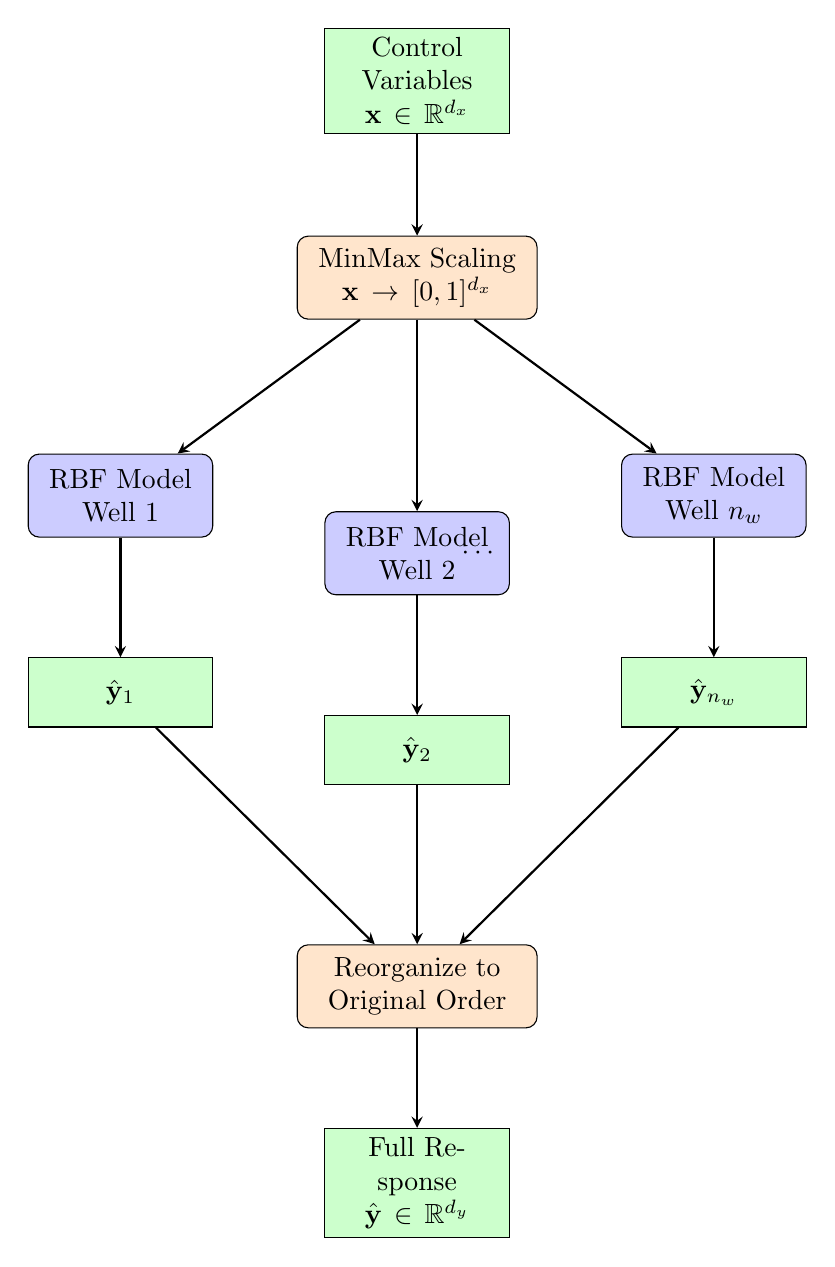
\begin{tikzpicture}[node distance=2.5cm]
    % Input
    \node (input) [data] {Control Variables $\mathbf{x} \in \mathbb{R}^{d_x}$};
    
    % Scaling
    \node (scale_x) [process, below of=input] {MinMax Scaling $\mathbf{x} \rightarrow [0,1]^{d_x}$};
    
    % Well models
    \node (well1) [block, below left of=scale_x, xshift=-2cm, yshift=-1cm] {RBF Model\\Well 1};
    \node (well2) [block, below of=scale_x, yshift=-1cm] {RBF Model\\Well 2};
    \node (welln) [block, below right of=scale_x, xshift=2cm, yshift=-1cm] {RBF Model\\Well $n_w$};
    \node (dots) [below of=scale_x, yshift=-1cm, xshift=0.8cm] {$\cdots$};
    
    % Outputs
    \node (out1) [data, below of=well1] {$\hat{\mathbf{y}}_1$};
    \node (out2) [data, below of=well2] {$\hat{\mathbf{y}}_2$};
    \node (outn) [data, below of=welln] {$\hat{\mathbf{y}}_{n_w}$};
    
    % Combine
    \node (combine) [process, below of=out2, yshift=-0.5cm] {Reorganize to Original Order};
    
    % Final output
    \node (final) [data, below of=combine] {Full Response $\hat{\mathbf{y}} \in \mathbb{R}^{d_y}$};
    
    % Arrows
    \draw [arrow] (input) -- (scale_x);
    \draw [arrow] (scale_x) -- (well1);
    \draw [arrow] (scale_x) -- (well2);
    \draw [arrow] (scale_x) -- (welln);
    \draw [arrow] (well1) -- (out1);
    \draw [arrow] (well2) -- (out2);
    \draw [arrow] (welln) -- (outn);
    \draw [arrow] (out1) -- (combine);
    \draw [arrow] (out2) -- (combine);
    \draw [arrow] (outn) -- (combine);
    \draw [arrow] (combine) -- (final);
\end{tikzpicture}
\caption{ProxyModelRBF architecture with well-based decomposition}
\end{figure}

\subsection{Data Flow}

The model processes data through the following stages:

\begin{enumerate}
    \item \textbf{Input Normalization}: Scale control variables $\mathbf{X}$ to $[0,1]$ using MinMax scaling
    \item \textbf{Well Decomposition}: Split output data $\mathbf{Y}$ by well identifier
    \item \textbf{Per-Well Scaling}: Apply MinMax scaling independently to each well's output
    \item \textbf{Per-Well RBF Training}: Train separate RBF interpolator for each well
    \item \textbf{Prediction}: For new inputs, predict each well independently
    \item \textbf{Reconstruction}: Combine well predictions into original data structure
\end{enumerate}

\section{Training Algorithm}

\begin{algorithm}
\caption{ProxyModelRBF Training}
\begin{algorithmic}[1]
\Require Training data $\mathbf{X} \in \mathbb{R}^{n \times d_x}$, $\mathbf{Y} \in \mathbb{R}^{n \times d_y}$
\Require Well names $\{w_1, w_2, \ldots, w_{n_w}\}$
\Require Kernel candidates $\mathcal{K} = \{\text{linear, cubic, gaussian, }\ldots\}$
\Ensure Trained RBF models $\{\hat{f}_{w_1}, \hat{f}_{w_2}, \ldots, \hat{f}_{w_{n_w}}\}$
\State
\State \textbf{// Step 1: Normalize inputs}
\State $\mathbf{X}_{\text{scaled}} \gets \text{MinMaxScale}(\mathbf{X}) \in [0,1]^{n \times d_x}$
\State
\State \textbf{// Step 2: Train-validation split}
\State $\mathbf{X}_{\text{train}}, \mathbf{X}_{\text{val}}, \mathbf{Y}_{\text{train}}, \mathbf{Y}_{\text{val}} \gets \text{TrainTestSplit}(\mathbf{X}_{\text{scaled}}, \mathbf{Y}, \text{test\_size}=0.1)$
\State
\State \textbf{// Step 3: Decompose by well}
\For{each well $w \in \{w_1, \ldots, w_{n_w}\}$}
    \State Extract $\mathbf{Y}^w_{\text{train}}$, $\mathbf{Y}^w_{\text{val}}$, $\mathbf{Y}^w$ from respective datasets
    \State $\mathbf{Y}^w_{\text{scaled}} \gets \text{MinMaxScale}(\mathbf{Y}^w)$
    \State $\mathbf{Y}^w_{\text{train,scaled}} \gets \text{Transform}(\mathbf{Y}^w_{\text{train}})$
    \State $\mathbf{Y}^w_{\text{val,scaled}} \gets \text{Transform}(\mathbf{Y}^w_{\text{val}})$
\EndFor
\State
\State \textbf{// Step 4: Kernel selection via cross-validation}
\For{each well $w \in \{w_1, \ldots, w_{n_w}\}$}
    \For{each kernel $\phi \in \mathcal{K}$}
        \State Train $\hat{f}_{\phi}$ using $\text{RBFInterpolator}(\mathbf{X}_{\text{train}}, \mathbf{Y}^w_{\text{train,scaled}}, \text{kernel}=\phi)$
        \State $\hat{\mathbf{Y}}^w_{\text{val}} \gets \hat{f}_{\phi}(\mathbf{X}_{\text{val}})$
        \State $\text{MSE}_{\phi} \gets \frac{1}{|\mathbf{X}_{\text{val}}|} \|\mathbf{Y}^w_{\text{val,scaled}} - \hat{\mathbf{Y}}^w_{\text{val}}\|^2$
    \EndFor
    \State $\phi^* \gets \arg\min_{\phi} \text{MSE}_{\phi}$
    \State Train final model: $\hat{f}_w \gets \text{RBFInterpolator}(\mathbf{X}_{\text{scaled}}, \mathbf{Y}^w_{\text{scaled}}, \text{kernel}=\phi^*)$
\EndFor
\State \Return $\{\hat{f}_{w_1}, \hat{f}_{w_2}, \ldots, \hat{f}_{w_{n_w}}\}$
\end{algorithmic}
\end{algorithm}

\section{Prediction Algorithm}

\begin{algorithm}
\caption{ProxyModelRBF Prediction}
\begin{algorithmic}[1]
\Require New control variables $\mathbf{x}^* \in \mathbb{R}^{d_x}$
\Require Trained models $\{\hat{f}_{w_1}, \ldots, \hat{f}_{w_{n_w}}\}$
\Ensure Predicted response $\hat{\mathbf{y}}^* \in \mathbb{R}^{d_y}$
\State
\State \textbf{// Step 1: Scale input}
\State $\mathbf{x}^*_{\text{scaled}} \gets \text{MinMaxTransform}(\mathbf{x}^*)$
\State
\State \textbf{// Step 2: Predict per well}
\For{each well $w \in \{w_1, \ldots, w_{n_w}\}$}
    \State $\hat{\mathbf{y}}^{*,w}_{\text{scaled}} \gets \hat{f}_w(\mathbf{x}^*_{\text{scaled}})$
    \State $\hat{\mathbf{y}}^{*,w} \gets \text{InverseMinMaxTransform}(\hat{\mathbf{y}}^{*,w}_{\text{scaled}})$
\EndFor
\State
\State \textbf{// Step 3: Reorganize to original data order}
\State $\hat{\mathbf{y}}^* \gets \text{Reorganize}(\{\hat{\mathbf{y}}^{*,w_1}, \ldots, \hat{\mathbf{y}}^{*,w_{n_w}}\})$
\State \Return $\hat{\mathbf{y}}^*$
\end{algorithmic}
\end{algorithm}

\section{Key Features and Advantages}

\subsection{Per-Well Independence}
\begin{itemize}
    \item Each well's response is modeled independently
    \item Allows different RBF kernels for different wells based on their characteristics
    \item Scalable to large number of wells
    \item Natural handling of well-specific dynamics
\end{itemize}

\subsection{Automatic Kernel Selection}
\begin{itemize}
    \item Evaluates 6 different RBF kernels per well
    \item Selects optimal kernel via 10\% validation split
    \item Minimizes mean squared error (MSE) on held-out data
    \item Prevents overfitting to training data
\end{itemize}

\subsection{Proper Scaling Strategy}
\begin{itemize}
    \item Input features scaled to $[0,1]$ for numerical stability
    \item Output scaling performed \textit{per well} to preserve relative magnitudes
    \item Independent scalers allow for different output ranges across wells
\end{itemize}

\subsection{Fast Predictions}
\begin{itemize}
    \item Once trained, provides near-instantaneous predictions
    \item Enables real-time optimization of control strategies
    \item Suitable for gradient-based optimization algorithms
    \item No need for expensive simulator calls during optimization
\end{itemize}

\section{Computational Complexity}

\subsection{Training Phase}
\begin{itemize}
    \item Data decomposition: $O(n \cdot d_y)$
    \item RBF interpolator construction per well: $O(n^3)$ (matrix inversion)
    \item Total with $n_w$ wells and $|\mathcal{K}|$ kernels: $O(|\mathcal{K}| \cdot n_w \cdot n^3)$
\end{itemize}

\subsection{Prediction Phase}
\begin{itemize}
    \item Per-well prediction: $O(n \cdot d_x)$ 
    \item Total with $n_w$ wells: $O(n_w \cdot n \cdot d_x)$
    \item Reorganization: $O(d_y)$
\end{itemize}

\section{Application in Closed-Loop Optimization}

\begin{figure}[h]
\centering
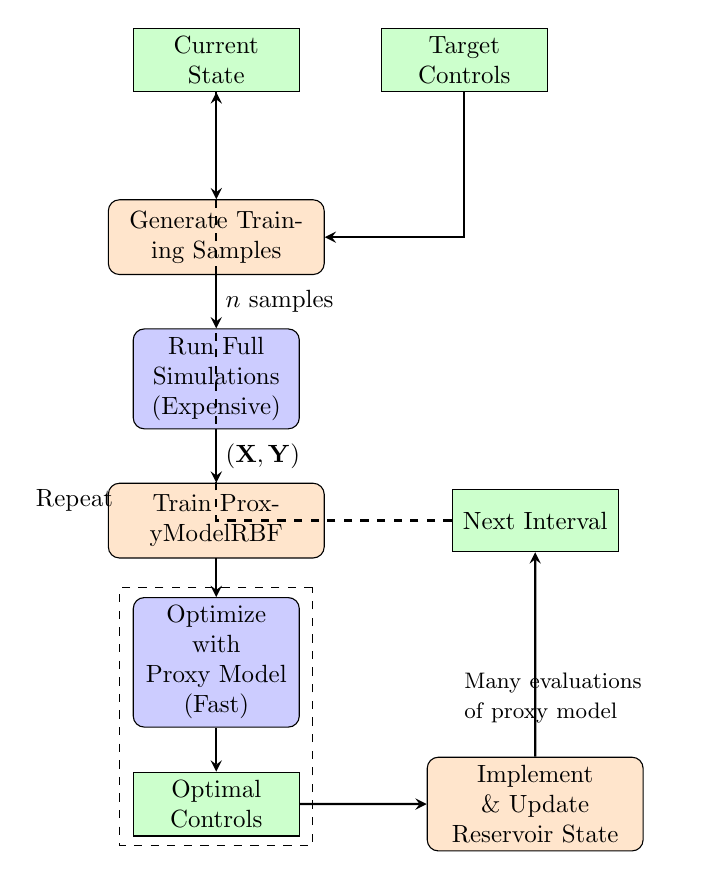
\begin{tikzpicture}[node distance=2cm, scale=0.9, every node/.style={scale=0.9}]
    % Nodes
    \node (current) [data] {Current State};
    \node (target) [data, right of=current, xshift=1.5cm] {Target Controls};
    \node (sample) [process, below of=current, yshift=-0.5cm] {Generate Training Samples};
    \node (simulate) [block, below of=sample] {Run Full Simulations\\(Expensive)};
    \node (train) [process, below of=simulate] {Train ProxyModelRBF};
    \node (optimize) [block, below of=train] {Optimize with\\Proxy Model\\(Fast)};
    \node (optimal) [data, below of=optimize] {Optimal Controls};
    \node (implement) [process, right of=optimal, xshift=2.5cm] {Implement \& Update\\Reservoir State};
    \node (next) [data, above of=implement, yshift=2cm] {Next Interval};
    
    % Arrows
    \draw [arrow] (current) -- (sample);
    \draw [arrow] (target) |- (sample);
    \draw [arrow] (sample) -- node[right] {$n$ samples} (simulate);
    \draw [arrow] (simulate) -- node[right] {$(\mathbf{X}, \mathbf{Y})$} (train);
    \draw [arrow] (train) -- (optimize);
    \draw [arrow] (optimize) -- (optimal);
    \draw [arrow] (optimal) -- (implement);
    \draw [arrow] (implement) -- (next);
    \draw [arrow, dashed] (next) -| node[above, xshift=-2cm] {Repeat} (current);
    
    % Annotation
    \node[draw, dashed, fit=(optimize) (optimal), inner sep=0.3cm] {};
    \node[right of=optimize, xshift=3cm, yshift=-0.5cm, text width=3cm, align=left] {\small Many evaluations\\of proxy model};
    
\end{tikzpicture}
\caption{ProxyModelRBF in closed-loop optimization workflow}
\end{figure}

The proxy model enables:
\begin{enumerate}
    \item \textbf{Rapid Training}: Uses $n \sim 100-1000$ expensive simulations
    \item \textbf{Efficient Optimization}: Thousands of proxy evaluations during optimization
    \item \textbf{Constraint Handling}: Fast evaluation of production/emission constraints
    \item \textbf{Multi-Interval Planning}: Re-train at each time interval with updated state
\end{enumerate}

\section{Implementation Details}

\subsection{Dependencies}
\begin{itemize}
    \item \texttt{scipy.interpolate.RBFInterpolator}: Core RBF interpolation
    \item \texttt{sklearn.preprocessing.MinMaxScaler}: Feature scaling
    \item \texttt{sklearn.model\_selection.train\_test\_split}: Validation split
    \item \texttt{sklearn.metrics.mean\_squared\_error}: Model evaluation
\end{itemize}

\subsection{Hyperparameters}
\begin{itemize}
    \item Shape parameter: $\epsilon = 1.0$ (fixed)
    \item Validation split: 10\% of training data
    \item Kernel candidates: 6 options (linear, cubic, thin plate spline, Gaussian, multiquadric, inverse multiquadric)
\end{itemize}

\section{Limitations and Considerations}

\begin{itemize}
    \item \textbf{Training Cost}: $O(n^3)$ scaling limits to moderate sample sizes ($n < 10,000$)
    \item \textbf{Extrapolation}: RBF interpolators may be unreliable outside training domain
    \item \textbf{Memory}: Stores all training points; memory scales as $O(n \cdot d_x)$
    \item \textbf{High Dimensions}: Performance may degrade in very high-dimensional input spaces
    \item \textbf{Smoothness}: Assumes smooth relationship between inputs and outputs
\end{itemize}

\section{Comparison with Alternative Approaches}

\begin{table}[h]
\centering
\begin{tabular}{|l|c|c|c|c|}
\hline
\textbf{Method} & \textbf{Training Time} & \textbf{Prediction Time} & \textbf{Accuracy} & \textbf{Scalability} \\ \hline
ProxyModelRBF & Medium & Very Fast & High & Good \\ \hline
Polynomial Regression & Fast & Very Fast & Low-Medium & Excellent \\ \hline
Gaussian Process & Slow & Medium & High & Poor \\ \hline
Neural Network & Slow & Fast & Medium-High & Excellent \\ \hline
Random Forest & Medium & Medium & Medium & Good \\ \hline
\end{tabular}
\caption{Comparison of surrogate modeling approaches}
\end{table}

\section{Conclusion}

The \texttt{ProxyModelRBF} provides an effective surrogate modeling strategy for reservoir optimization problems by:
\begin{itemize}
    \item Decomposing the problem by well for better scalability
    \item Automatically selecting optimal kernels per well
    \item Providing fast, accurate predictions for optimization
    \item Maintaining interpretability through well-based structure
\end{itemize}

This approach balances computational efficiency with prediction accuracy, making it suitable for closed-loop optimization frameworks where repeated training and prediction cycles are required.

\end{document}
